% CVPR 2026 Paper Template; see https://github.com/cvpr-org/author-kit

\documentclass[10pt,twocolumn,letterpaper]{article}
%\usepackage{times}
%%%%%%%%% PAPER TYPE  - PLEASE UPDATE FOR FINAL VERSION
% \usepackage{cvpr}              % To produce the CAMERA-READY version
\usepackage[review]{cvpr}      % To produce the REVIEW version
% \usepackage[pagenumbers]{cvpr} % To force page numbers, e.g. for an arXiv version

% Import additional packages in the preamble file, before hyperref
\input{preamble}

% It is strongly recommended to use hyperref, especially for the review version.
% hyperref with option pagebackref eases the reviewers' job.
% Please disable hyperref *only* if you encounter grave issues, 
% e.g. with the file validation for the camera-ready version.
%
% If you comment hyperref and then uncomment it, you should delete *.aux before re-running LaTeX.
% (Or just hit 'q' on the first LaTeX run, let it finish, and you should be clear).
\definecolor{cvprblue}{rgb}{0.21,0.49,0.74}
\usepackage[pagebackref,breaklinks,colorlinks,allcolors=cvprblue]{hyperref}

%%%%%%%%% PAPER ID  - PLEASE UPDATE
\def\paperID{*****} % *** Enter the Paper ID here
\def\confName{CVPR}
\def\confYear{2026}

%%%%%%%%% TITLE - PLEASE UPDATE
\title{Generative Adversarial Networks for Data Augmentation and Domain Adaptation}

%%%%%%%%% AUTHORS - PLEASE UPDATE
\author{Mario De Paola\\
Politecnico di Torino\\
{\tt\small s334090@studenti.polito.it}
% For a paper whose authors are all at the same institution,
% omit the following lines up until the closing ``}''.
% Additional authors and addresses can be added with ``\and'',
% just like the second author.
% To save space, use either the email address or home page, not both
\and
Tommaso Centonze\\
Politecnico di Torino\\
{\tt\small s338411@studenti.polito.it}
}

\begin{document}
\maketitle
\begin{abstract}
La scarsità di dati etichettati e lo sbilanciamento delle classi rappresentano ostacoli critici nello sviluppo di modelli di Deep Learning per la diagnostica medica. Questo lavoro esplora l'efficacia delle Generative Adversarial Networks (GAN) come strumento di data augmentation per migliorare la classificazione della polmonite in immagini radiografiche pediatriche \cite{kermany2018identifying}. Utilizzando un dataset intrinsecamente sbilanciato, proponiamo l’impiego di una Conditional Deep Convolutional Wasserstein GAN con Gradient Penalty (cDC-WGAN-GP), sintetizzando i contributi fondamentali di \cite{mirza2014conditionalgenerativeadversarialnets}, \cite{radford2015unsupervised}, \cite{arjovsky2017wasserstein} e \cite{gulrajani2017improved}. Una ResNet18 \cite{He_2016_CVPR} viene utilizzata come classificatore baseline e successivamente addestrata sul dataset aumentato. I risultati indicano che l'integrazione di campioni sintetici della classe minoritaria permette di ottimizzare l'F1-score, riducendo la polarizzazione del modello. [...continue DA...].
\end{abstract}    
\section{Introduction}
\label{sec:intro}

L'interpretazione automatizzata delle radiografie del torace (CXR) è diventata un pilastro della radiologia assistita dal computer. Tuttavia, l'efficacia dei modelli allo stato dell'arte è strettamente legata alla disponibilità di dataset bilanciati. Il dataset pediatrico "Chest X-Ray Pneumonia" \cite{kermany2018identifying} presenta uno sbilanciamento di circa 1:3 tra casi sani (NORMAL) e casi patologici (PNEUMONIA). In tali scenari, un classificatore basato su architetture residue come la ResNet18 \cite{He_2016_CVPR} tende a massimizzare l'accuratezza globale a discapito della capacità di identificare correttamente la classe minoritaria, portando a un F1-score sub-ottimale.

Per ovviare a queste limitazioni, questo progetto implementa una strategia di Data Augmentation generativa. Invece di limitarsi a trasformazioni geometriche, abbiamo progettato una cDC-WGAN-GP. Questa architettura combina il condizionamento delle etichette \cite{mirza2014conditionalgenerativeadversarialnets} con la stabilità della Wasserstein Loss \cite{arjovsky2017wasserstein} e della Gradient Penalty \cite{gulrajani2017improved}, permettendo di generare immagini radiografiche sintetiche che catturano la distribuzione della classe sottorappresentata. L'obiettivo finale è dimostrare come l'arricchimento del dataset possa fungere da regolarizzatore e migliorare la generalizzazione. Inoltre, il lavoro esplora l'impatto di tali tecniche in scenari di domain adaptation. [...continue DA...].


\section{Related Work}
\label{sec:Related_Works}

La letteratura recente nell'ambito della visione artificiale applicata alla medicina ha visto una convergenza tra architetture di classificazione profonda e modelli generativi.

\subsection{Classificazione e Residual Learning}

Il riconoscimento d'immagini moderno è dominato dalle Residual Networks introdotte da He et al. \cite{He_2016_CVPR}. La loro capacità di addestrare reti molto profonde tramite connessioni shortcut ha permesso di raggiungere performance d'eccellenza anche nel dominio medico. Nel contesto specifico delle radiografie toraciche, il lavoro di Kermany et al. \cite{kermany2018identifying} ha stabilito un benchmark fondamentale, dimostrando come modelli pre-addestrati possano assistere i clinici nella diagnosi della polmonite pediatrica.

\subsection{Evoluzione delle Generative Adversarial Networks}

Le GAN hanno rivoluzionato la generazione di dati sintetici. Le Deep Convolutional GAN (DCGAN) \cite{radford2015unsupervised} hanno introdotto vincoli architettonici basati su livelli convoluzionali che hanno reso possibile la generazione di immagini coerenti. Per permettere una generazione mirata alle classi specifiche, Mirza e Osindero \cite{mirza2014conditionalgenerativeadversarialnets} hanno proposto le Conditional GAN (cGAN), estendendo l'architettura per includere informazioni supplementari come input sia per il generatore che per il discriminatore.

\subsection{Addestramento Stabile e Wasserstein GAN}

Uno dei problemi storici delle GAN è l'instabilità dell'addestramento. La Wasserstein GAN (WGAN) \cite{arjovsky2017wasserstein} ha affrontato questo problema sostituendo la divergenza di Jensen-Shannon con la distanza di Earth-Mover, fornendo un gradiente più informativo. Per superare le limitazioni del weight clipping originariamente proposto, Gulrajani et al. \cite{gulrajani2017improved} hanno introdotto la Gradient Penalty (WGAN-GP), garantendo il rispetto del vincolo di Lipschitz in modo più fluido e robusto. L'unione di queste tecniche rappresenta l'attuale stato dell'arte per la generazione di immagini mediche ad alta fedeltà.

Le potenzialità di queste immagini sintetiche si estendono anche al superamento delle discrepanze tra dataset di diversa provenienza. [...continue DA...].

\section{Methodology}

Il cuore del progetto risiede in una pipeline sequenziale progettata per validare l'ipotesi che la generazione sintetica mirata possa mitigare i limiti strutturali di un dataset sbilanciato.

\subsection{Fase 1: Valutazione della Baseline e Analisi dello Sbilanciamento}

Il punto di partenza del lavoro consiste nello stabilire un benchmark di riferimento attraverso l'addestramento di un classificatore ResNet18 sul dataset originale. In questa fase, l'enfasi è posta sull'identificazione del bias indotto dallo sbilanciamento di classe (circa 3:1).\\

Data la natura critica della diagnostica medica, abbiamo scelto di non affidarci all'accuratezza globale, metrica che in presenza di classi minoritarie risulta spesso ingannevole. Abbiamo invece adottato il Macro F1-Score come bussola per la valutazione: questa metrica, calcolando la media non pesata delle armoniche tra precisione e richiamo di ogni classe, costringe il modello a dimostrare competenza anche sulla classe NORMAL, impedendo alla rete di ignorare i casi sani per massimizzare il successo statistico sui casi di polmonite.

\subsection{Fase 2: Implementazione della C-DCWGAN-GP}

Per colmare il gap distributivo, abbiamo optato per un framework generativo avanzato che potesse garantire non solo il realismo visivo, ma anche la stabilità numerica.

L'architettura scelta è una Conditional Deep Convolutional WGAN-GP. L'aspetto condizionale è fondamentale: integrando l'encoding One-Hot delle etichette direttamente nel vettore latente $N_z = 100$, permettiamo al generatore di apprendere una rappresentazione disaccoppiata delle due classi. Dal punto di vista della stabilità, abbiamo abbandonato le GAN classiche in favore della formulazione di Wasserstein. La stabilità è ulteriormente blindata dalla Gradient Penalty (GP), la quale impone il vincolo di 1-Lipschitz continuity necessario per un addestramento fluido.\\

Un aspetto distintivo della nostra implementazione riguarda la gestione del Critic. Per evitare che la Gradient Penalty venisse corrotta da dipendenze inter-campione, abbiamo rimosso ogni strato di Batch Normalization nel Critic, sostituendolo con la Layer Normalization. Inoltre, per prevenire derive numeriche nelle fasi avanzate di training, abbiamo introdotto una Epsilon Drift Penalty, una sorta di "ancora" matematica che mantiene i valori di output del Critic entro range computazionalmente sicuri.

\subsection{Fase 3: Validazione "In-Loop" e Valutazione Finale}

La selezione del generatore ottimale non è stata lasciata al caso o a una valutazione puramente estetica. Abbiamo implementato un sistema di Augmented Validation: ad intervalli regolari, una ResNet "sonda" viene addestrata su un mix di dati reali e campioni sintetici appena prodotti. Solo il checkpoint della GAN che permette alla sonda di ottenere il miglior Macro F1-Score sul validation set reale viene scelto per la fase finale. In quest'ultima fase, il dataset viene portato a un rapporto di equilibrio 1:1, addestrando il classificatore definitivo per dimostrare come la diversità sintetica si traduca in una superiore capacità di generalizzazione.
\section{Experimental Setup}

Per garantire la replicabilità del lavoro, l'addestramento è stato meticolosamente calibrato seguendo le best practice del deep learning generativo.

\subsection{Ribilanciamento dei Set di Valutazione}

Un limite critico riscontrato nel dataset originale riguardava la partizione di validazione ufficiale, composta da soli 16 campioni. Tale dimensione esigua rendeva le metriche di validazione statisticamente insignificanti e soggette a fluttuazioni estreme durante l'addestramento. 

Per ovviare a questo problema, è stata effettuata una procedura di \textit{stratified re-sampling}. Il validation set originale è stato aumentato prendendo il 12.5\% del test set. Questa ridistribuzione ha garantito che sia il set di validazione che quello di test mantenessero la proporzione originale delle classi, fornendo al contempo una base statistica sufficientemente ampia per monitorare accuratamente la convergenza del modello e prevenire l'overfitting.

\subsection{Dinamiche di Ottimizzazione e Parametri della GAN}

La C-DCWGAN-GP opera su immagini standardizzate a una risoluzione di 128x128 pixel. L'addestramento, esteso per un arco di 100 epoche, segue una dinamica asincrona: il Critic viene aggiornato con una frequenza di 5 a 1 rispetto al Generatore $(n_{critic} = 5)$

Questo squilibrio controllato assicura che il Generatore riceva sempre gradienti densi e ben definiti da un "avversario" vicino all'ottimalità.

L'ottimizzatore Adam è stato configurato con un learning rate iniziale di $10^{-4}$ e coefficienti di momentum impostati a $\beta_1 = 0.0$ e $\beta_2 = 0.9$. L'azzeramento di $\beta$ è una scelta deliberata per eliminare l'inerzia dei gradienti storici, permettendo al modello di reagire istantaneamente ai rapidi cambiamenti del Critic. La convergenza finale è assistita da un MultiStepLR scheduler, che riduce il learning 
rate del 80\% (fattore $\gamma = 0.2$) alle epoche 60 e 80, permettendo una sintonizzazione fine delle feature microscopiche nelle radiografie.

\subsection{Training del Classificatore}

I classificatori ResNet (sia quello baseline che quello finale) sono stati addestrati con una strategia più conservativa: 10 epoche con una batch size di 32 e un learning rate fisso di 0.001. Questa configurazione è stata scelta per isolare l'effetto della qualità dei dati (l'augmentation) rispetto alla complessità dell'ottimizzazione, mantenendo un ambiente di test controllato e confrontabile.
\section{Risultati e Discussione}

In questa sezione vengono analizzati i risultati ottenuti, confrontando un approccio preliminare basato su una GAN incondizionata con il sistema C-DCWGAN-GP finale.

\subsection{Analisi Preliminare: Il problema della scarsità di dati}

Inizialmente, è stato condotto un esperimento per testare la capacità di  apprendere la distribuzione della sola classe minoritaria, utilizzando esclusivamente i 1341 campioni reali disponibili. 
I risultati sono stati insoddisfacenti: la rete non è stata in grado di convergere verso una rappresentazione realistica, producendo immagini affette da artefatti evidenti e segnali di mode collapse. L'integrazione di questi campioni nel dataset di addestramento ha portato a un degrado delle performance della ResNet18. Questo fallimento conferma un'ipotesi critica: una GAN necessita di una massa critica di dati per mappare correttamente le feature spaziali. Limitando il training alle sole immagini sane, il modello non ha beneficiato del confronto con le caratteristiche morfologiche della polmonite, fallendo nel definire i confini della classe.

\begin{figure}[ht]
    \centering
    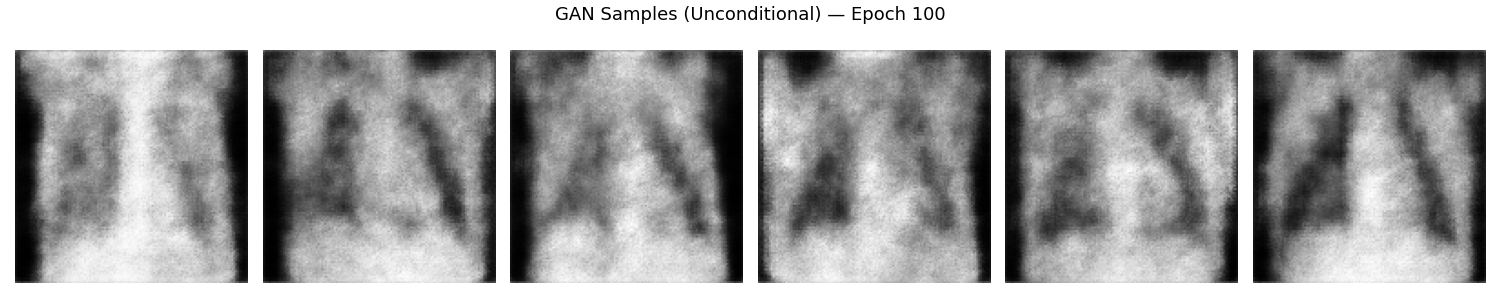
\includegraphics[width=\columnwidth]{images/samples_epoch_100_uncond.png} 
    \caption{Evoluzione dei campioni generati per il modello incondizionato.}
    \label{fig:samples_unconditional}
\end{figure}

\subsection{Risultati Finali: Data Augmentation tramite C-DCWGAN-GP}

L'adozione della Conditional GAN, addestrata sull'intero pool di dati, ha ribaltato i risultati. Sfruttando le informazioni provenienti da entrambe le classi, il generatore ha prodotto campioni sintetici di alta qualità che hanno permesso un bilanciamento efficace del dataset.

\paragraph{Analisi Quantitativa}
Il confronto tra la Baseline (Phase 1) e il modello addestrato con i dati sintetici (Phase 3) evidenzia un netto miglioramento in tutte le metriche chiave \ref{fig:cm1}, \ref{tab:confronto_classi}.

\begin{figure}[ht]
    \centering
    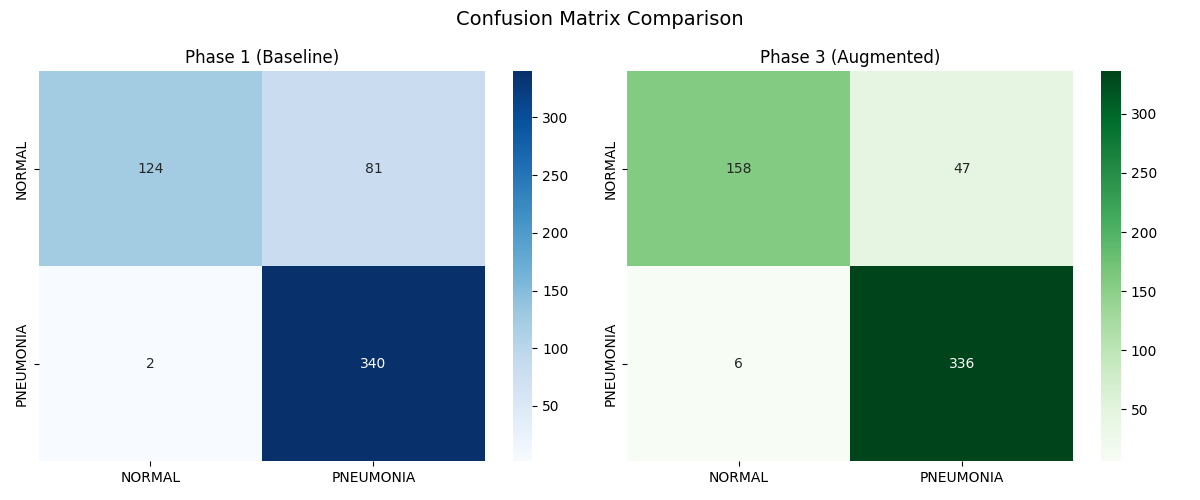
\includegraphics[width=\columnwidth]{images/cm_comparison-4.png} 
    \caption{Confronto tra matrici di confusioni baseline vs augmented.}
    \label{fig:cm1}
\end{figure}

\begin{table}[h]
\centering
\resizebox{\columnwidth}{!}{%
    \begin{tabular}{l|cc|cc}
    \toprule
    & \multicolumn{2}{c|}{\textbf{Normal}} & \multicolumn{2}{c}{\textbf{Pneumonia}} \\ 
    \textbf{Modello} & Rec. & F1 & Prec. & F1 \\ \midrule
    Baseline & 0.60 & 0.74 & 0.80 & 0.89 \\
    \textbf{Augm.} & \textbf{0.77} & \textbf{0.85} & \textbf{0.87} & \textbf{0.92} \\ \midrule
    \textit{Delta} & +16\% & +11\% & +7\% & +3\% \\ \bottomrule
    \end{tabular}%
}
\caption{Confronto prestazioni per classe: Baseline vs Augmented (Phase 3). Si osserva il significativo recupero di Recall nella classe minoritaria.}
\label{tab:confronto_classi}
\end{table}

\begin{figure*}[t]
    \centering
    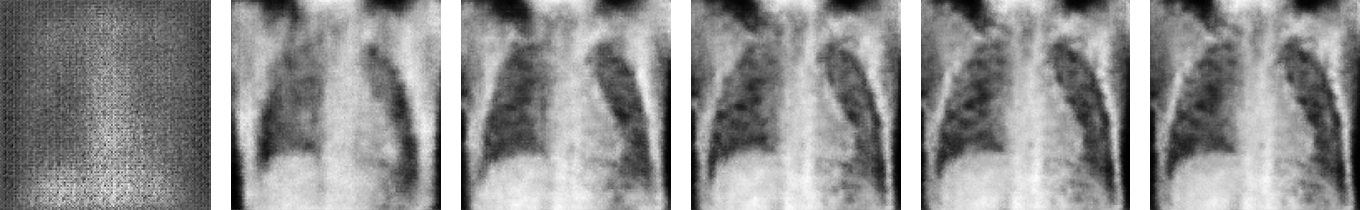
\includegraphics[width=\textwidth]{images/progressione_gan.png} 
    \caption{Progressione dell'addestramento della C-DCWGAN-GP: campioni generati ogni 20 epoche. Si osserva il passaggio dal rumore iniziale alla definizione dei dettagli anatomici polmonari.}
    \label{fig:progressione_completa}
\end{figure*}

Il dato più significativo è l'incremento del Recall per la classe NORMAL (da 0.60 a 0.77). Questo indica che il modello originale tendeva a classificare erroneamente molti pazienti sani come malati (falsi positivi), a causa della scarsa rappresentazione dei polmoni sani nel training set. L'introduzione di dati sintetici ha permesso alla ResNet18 di imparare a distinguere con molta più precisione le sottili differenze visive, portando l'accuratezza globale oltre il 90%.

\subsection{Analisi Qualitativa e Training Stability}

L'analisi dei log di Weights  Biases (WandB) ha confermato la stabilità della C-DCWGAN-GP. A differenza dell'esperimento 1, la Wasserstein Loss ha mostrato una decrescita regolare, correlata visivamente a un progressivo miglioramento dei campioni generati.

I sample generati \ref{fig:progressione_completa} mostrano una corretta ricostruzione delle strutture costali e dei campi polmonari, confermando che il condizionamento della label e l'aumento dei dati di training totali hanno permesso al modello di superare i limiti della scarsità di dati iniziale.


{
    \small
    \bibliographystyle{ieeenat_fullname}
    \bibliography{main}
}

% WARNING: do not forget to delete the supplementary pages from your submission 
% \input{sec/X_suppl}

\end{document}
